\documentclass[xcolor=dvipsnames,smaller]{beamer}
\usepackage[latin1]{inputenc}
\usepackage{colortbl}
\usepackage{beamerthemesplit}
\usepackage{xmpmulti}
\usepackage{graphicx}
\usepackage{graphics}
\usepackage{wrapfig}
\usepackage{ulem}
\usepackage[T1]{fontenc}
\usepackage[latin1]{inputenc}
\usepackage{color}
\usepackage{amsmath}
\usepackage{amssymb}
\usepackage{amsthm}
\usepackage{epsfig,color,colordvi,wasysym}
%\usepackage{lineno}
\usepackage{setspace}
\usepackage{pdfpages}
\usetheme{Warsaw}
\usepackage{hyperref}

\setbeamertemplate{headline}{\vspace{0.cm}}
\setbeamertemplate{navigation symbols}{}
\setbeamertemplate{footline}{}
%\setbeamertemplate{background canvas}[default][top=SkyBlue]
\setbeamertemplate{background canvas}{}
\setbeamertemplate{frametitle}[shadow theme]
\setbeamercolor{frametitle}{fg=white, bg=Blue}
\setbeamertemplate{theorems}[default]
%\setbeamercolor{block title}{fg=DarkBlue, bg=Tan} 
%\setbeamercolor{block body}{bg=Tan} 
%\setbeamersize{text margin left=0em,text margin right=0em}
%\setbeamertemplate{frametitle}{}  %Removes the frametitle from each slide


\title[BBM402-Lecture 1: Turing Machines]
{BBM402-Lecture 1: Turing Machines}
\author{
\vspace{2cm}
%\hspace{-1cm}
\textcolor{Blue}{\large{Lecturer: Lale \"Ozkahya}}}
\date{
\footnotesize{
Resources for the presentation:\\
https://courses.engr.illinois.edu/cs373/fa2010/lectures\\
https://courses.engr.illinois.edu/cs498374/lectures.html}}

\begin{document}

\newtheorem{thm}[theorem] {Theorem}
\newtheorem{lem}[theorem]{Lemma}
\newtheorem{cor}[theorem]{Corollary}
\newtheorem{prp}[theorem]{Proposition}
\newtheorem{clm}[theorem]{Claim}
\newtheorem{conj}[theorem]{Conjecture}
\newtheorem{remark}[theorem]{Remark}
\newtheorem{construction}[theorem]{Construction}

\def\EE{\mathcal{E}}


\def\tr{\textcolor{Red}}
\def\tb{\textcolor{Blue}}
\def\vs{\vspace{0.5cm}}

\begin{frame}
\titlepage
\end{frame}

\normalsize{

%\begin{frame}\frametitle{Course Information}
%\begin{center}
%{\bf 
%\href{http://web.cs.hacettepe.edu.tr/~ozkahya/bbbm402/index.html}
%{http://web.cs.hacettepe.edu.tr/~ozkahya/bbbm402/index.html}
%} 
%\end{center}
%\end{frame}

\includepdf[pagecommand={\thispagestyle{empty}}, 
pages=2-83, angle=0, scale = 1.]{BBM401Turing-mach.pdf}

}
\end{document}


